\documentclass[anonymous,12pt]{iopjournal}
\usepackage{amsmath,amssymb,amsthm,booktabs,array}
\usepackage{microtype}
\usepackage{graphicx,placeins}
\graphicspath{{figures/}}
\hypersetup{hidelinks,pdftitle={Certifying peak dielectric contrast from finite-aperture scattering data},pdfauthor={}}
\fancyhead[L]{\small\sffamily Inverse Problems\quad Research paper}
\fancyhead[R]{\small Peak contrast from finite-aperture data}
\newtheorem{theorem}{Theorem}[section]
\newtheorem{proposition}[theorem]{Proposition}
\newtheorem{lemma}[theorem]{Lemma}
\newtheorem{corollary}[theorem]{Corollary}
\theoremstyle{remark}\newtheorem{remark}[theorem]{Remark}
\newcommand{\C}{\mathbb C}\newcommand{\R}{\mathbb R}
\newcommand{\Herm}{\operatorname{Re}_{\!H}}\newcommand{\Imag}{\operatorname{Im}_{\!H}}
\newcommand{\tr}{\operatorname{tr}}\newcommand{\diag}{\operatorname{diag}}
\newcommand{\rank}{\operatorname{rank}}\newcommand{\dist}{\operatorname{dist}}
\newcommand{\Dpos}{D_{\mu}}\newcommand{\Dopt}{D_{\lambda}}
\newcommand{\abs}[1]{\left|#1\right|}\newcommand{\norm}[1]{\left\|#1\right\|}
\newcommand{\eps}{\varepsilon}\newcommand{\dd}{\mathrm{d}}
\newcommand{\citep}[1]{\cite{#1}}
\numberwithin{equation}{section}
\setlength{\emergencystretch}{1.8em}
\setcounter{topnumber}{3}\setcounter{bottomnumber}{2}
\renewcommand{\topfraction}{.9}\renewcommand{\textfraction}{.09}
\begin{document}
\noindent{\sffamily\small RESEARCH PAPER}\par\vspace{1.8ex}
\title{Certifying peak dielectric contrast from finite-aperture scattering data: optical power and negative inertia across illuminations}
\author{}
\begin{abstract}
A finite receiver array can measure a scattered field accurately while leaving large internal currents undetermined. We use the joint response to several incident waves to bound the peak of an unknown lossless dielectric without initializing a reconstruction. The sector and optical matrix balances characterize the shared constitutive law when enforced pixelwise on actual currents. A weighted combination gives a lower bound on the distance from measured data to all media below a prescribed contrast. Each negative state direction can remove at most one term from this bound. We construct exact coherent fits by adding receiver-invisible currents that restore both global balances, even when the joint bound excludes the contrast cap. Outward-rounded calculations retain all 9,216 material variables in a two-dimensional transverse-magnetic model. On six strong scatterers, half-aperture data establish peak contrast above 0.5 in six cases at 2\% noise and three at 10\%. At a peak threshold of 0.75, the full ring gives strict separations on three objects at 1\% noise and two at 2\%. On the latter two observations a four-region single-source semidefinite relaxation has zero optimal distance for every coherent input under any uniform current-energy cap valid throughout the material box. Sixteen regions recover both exclusions with a single coherent direction. Frozen bounds transfer to 22 additional scatterers at threshold 0.5 and to five of seven scatterers at threshold 5 on a second array. Independent microwave-chamber measurements quantify the discrepancy still allowable after changing the calibration reference.
\end{abstract}
\keywords{inverse electromagnetic scattering, contrast source, optical theorem, finite aperture, semidefinite relaxation, inertia, uncertainty bounds}

\section{Introduction}\label{sec:intro}

Suppose a reconstruction assigns a small dielectric contrast to every point in the imaging region. Can the measurements rule out \emph{all} materials with such a small peak? Evaluating the residual of the proposed image answers this question for one image. A high residual leaves open the possibility that a different arrangement of the same low-contrast material fits perfectly. A lower bound on the residual over the whole contrast box answers the stronger question. It can remain useful when the data cannot specify where the dielectric is located.

Reconstruction and exclusion use the same wave equation but answer different questions. Classical scattering theory gives the forward field for a specified medium \cite{colton}; computational methods then use the data to estimate that medium \cite{chenbook}. Contrast-source inversion updates internal sources and contrast jointly \cite{csi}. Alternative integral equations change the variables used to estimate strongly scattering media \cite{nie,cie}. An image produced by any of these methods can be tested against the same peak-contrast hypothesis.

The distinction starts in current space. At one frequency the receiver samples the induced contrast current through a linear operator $S$. A particular fit of a noiseless single-source datum can be augmented by any element of $\ker S$. Subspace-based inversion exploits the measured current components before optimizing the components poorly determined by the receiver \cite{chen,zhong}. A current invisible to a finite receiver array can still radiate power outside the array. Conversely, sufficiently dense reception can account for essentially all the radiated power of some discretizations, although the material inference still has a large current null space. The optical theorem has different consequences in these two settings. The relevant quantity is the radiation operator restricted to $\ker S$, with the actual frequency and receiver normalization.

A finite receiver null space also has a different physical meaning from a non-scattering wave. The latter concerns an incident field and a medium whose scattered far field vanishes in every direction. Transmission eigenfunctions and boundary regularity constrain when that can happen \cite{cakoni_book,cakoni_vogelius}. A current in $\ker S$ need only vanish at the sampled receivers. A direct measure of how much power can still escape those receivers enters our bound in section~\ref{sec:single}.

Different incident waves produce different currents, but all of them must be compatible with the same real material at each location. This produces restrictions on their cross products. For one illumination, an invisible current may pay for a violation of a quadratic constraint without changing any receiver reading. With $s$ illuminations, the same indefinite state form must account for an $s$-by-$s$ matrix of violations. A form with four negative directions can accommodate at most four independent negative directions in any such current Gram. We exploit the surviving source spectrum to put a lower bound on a data distance in the original field units. No support map, material starting guess or reconstruction is needed for this test.

Several parts of this argument have established precedents. Trivedi et al. derived bounds for convex scattered-field objectives in lossless photonic structures \cite{trivedi}. Angeris et al. had already obtained computable performance bounds for photonic design objectives, including distance to a desired field \cite{angeris19}. Molesky et al. used real and reactive power conservation together and subsequently imposed regional constraints in a hierarchy of scattering bounds \cite{moleskyglobal,moleskylocal}. Kuang and Miller obtained scattering limits from local conservation laws in a volume-integral formulation \cite{kuang}. Angeris et al. studied attainable device performance by comparing photonic designs with optimization bounds \cite{angeris}. Cross-excitation constraints for a common material structure are central in the multifunctional bounds of Shim et al. \cite{shim}. The extremal inertia of a Hermitian matrix quadratic is a matrix-analysis problem in its own right; Tian gives a related exact identity in Corollary~4.5, equation~(4.38), for a matrix quadratic with a solvable cancellation equation \cite{tian}. Finite-dimensional exceptions to positivity also occur in continuous Maxwell inverse scattering. Griesmaier and Harrach used far-field monotonicity for the support of penetrable acoustic scatterers \cite{griesmaier_harrach,griesmaier_harrach_erratum}. Albicker and Griesmaier developed a corresponding support characterization for Maxwell fields \cite{albicker}. Their operator, data and inverse task differ from the finite-port contrast-box residual considered here.

An indefinite state form still yields an evaluable bound on the measured distance. We construct exact single-source witnesses for both global laws and compare the resulting separation against regional relaxations. A one-sided Fourier bound reduces the proof matrix while retaining every material variable. A current that fits one datum may fail the constitutive law; a positive exclusion covers every material satisfying it. The experiments quantify this distinction for simulated and measured fields.

\section{A joint data bound for a shared material}\label{sec:joint}

\subsection{Measurement model and quantifiers}
Let $n$ be the number of state and material cells, $s$ the number of incident waves, and $p$ the number of receiver positions common to these waves. Let $B\in\C^{n\times s}$ contain the incident fields, $G\in\C^{n\times n}$ the fixed background volume-integral operator, $S\in\C^{p\times n}$ the receiver matrix, and $Y\in\C^{p\times s}$ the measured scattered field. The contrast $M=\diag(m_i)$ is dimensionless, with $m_i=\epsilon_{r,i}-1$ for the nonmagnetic lossless dielectric model. The induced current and total field solve
\begin{equation}
 E=B+GJ,\qquad J=ME,\qquad F(M)=SJ. \label{eq:vie}
\end{equation}
The test applies to every solution of \eqref{eq:vie} for which the currents exist. It does not use a Born expansion or require a uniform bound on a forward inverse in deriving its lower bound. The scalar TM model retains multiple scattering to all orders resolved by the discretization. A vector analogue would require the corresponding tensor constitutive inequalities and compatible quadrature weights.

Let $U=\diag(u_i)$ be a proposed material upper bound, and let $r$ bound the joint data error in Frobenius norm. The admissible hypotheses have $0\le M\le U$. When $U=uI$, ruling out this entire box implies $\max_i m_i>u$ for every admissible material fitting the observations. This inference is conditional on nonemptiness of the larger physical feasible set if it is read as a statement about a particular experiment. We independently verify nonemptiness for the synthetic fine-grid tests. In the measured experiment we instead report the error budget under which the implication would apply.

For any square matrix $W$ write $\Herm W=(W+W^*)/2$ and $\Imag W=(W-W^*)/(2\mathrm i)$. For diagonal real weights $\Dpos\succeq0$ and $\Dopt$, the constitutive law implies
\begin{align}
 Q_{\rm r}(J)&=J^*\Dpos J-\Herm(J^*\Dpos U E)
       =E^*\Dpos M(M-U)E\preceq0,\label{eq:sector}\\
 Q_{\rm o}(J)&=\Imag(J^*\Dopt E)=0.\label{eq:optical}
\end{align}
The diagonal constraints commute with $M$. Testing the two matrices on an arbitrary $a\in\C^s$ tests the same identities for the incident field $Ba$ and current $Ja$. The off-diagonal entries keep precisely the restrictions that are lost when each original column is processed separately. For a lossless medium the signs of $D_{\lambda,ii}$ are unrestricted. In the sign convention of \eqref{eq:vie}, passive loss $\Im m_i\ge0$ changes \eqref{eq:optical} to a nonpositive form for $\Dopt\succeq0$. The real inequality simultaneously requires $|m_i|^2\le u_i\Re m_i$. A bound on $\Re m_i$ alone would be insufficient.

\subsection{The surviving source spectrum}
Set
\begin{align}
 Z&=(\Dpos U+\mathrm i\Dopt)/2,\nonumber\\
 K&=S^*S+\Dpos-ZG-G^*Z^*,\qquad L=S^*Y+ZB. \label{eq:operators}
\end{align}
For $K$ nonsingular write $H_Y=Y^*Y-L^*K^{-1}L$. Denote the negative index by $n_-(K)$ and the descending eigenvalues of $H_Y$ by $h_1\ge\cdots\ge h_s$. The subscript on $H_Y$ emphasizes that the final spectrum depends on the values of the data. Counting negative directions in $K$ alone cannot decide whether a material bound is informative.

\begin{theorem}[Noisy joint contrast bound]\label{th:bound}
If \eqref{eq:sector}--\eqref{eq:optical} hold and $K$ is nonsingular, then
\begin{equation}
 \norm{SJ-Y}_F^2\ \ge\ d^2(U,\Dpos,\Dopt;Y)
   :=\sum_{j=\nu+1}^{s}(h_j)_+,\qquad \nu=n_-(K), \label{eq:bound}
\end{equation}
where $(h)_+=\max(h,0)$ and an empty sum is zero. Consequently, $d>r$ is sufficient to exclude the material box. This inequality applies to any fixed admissible multipliers, including ones proposed using $Y$.
\end{theorem}
\begin{proof}
Let $D=(SJ-Y)^*(SJ-Y)$, which is positive semidefinite. Adding $Q_{\rm r}+Q_{\rm o}$ to $D$ gives
\begin{equation}
 D\succeq Y^*Y-J^*L-L^*J+J^*KJ
 =H_Y+(J-K^{-1}L)^*K(J-K^{-1}L).\label{eq:complete}
\end{equation}
The negative part of the last congruence has rank at most $\nu$. For $i+\nu\le s$, rank interlacing gives $\lambda_i(D)\ge h_{i+\nu}$. Each $\lambda_i(D)$ is also nonnegative. Summing proves \eqref{eq:bound}. All identities hold for the actual $J$; optimizing over proposed weights can only strengthen the resulting lower bound. Numerical proposals used in the experiments are checked separately by outward rounding.
\end{proof}

The formula has a precise sense of sharpness. Free the residual Gram and state deviation in \eqref{eq:complete}, retaining just $D\succeq0$ and $D\succeq H_Y+X^*KX$ for a freely chosen $X$. The minimum of $\tr D$ over these two inequalities equals \eqref{eq:bound}. Indeed a basis of the negative subspace of $K$ can be rescaled to have Gram $-I_\nu$. Using up to $\nu$ of these directions cancels the largest positive eigenvalues of $H_Y$ exactly. Taking the positive part of the remainder attains the stated trace. Equality for this free epigraph does not identify a current that solves \eqref{eq:vie}. It explains which information has already been exhausted when a selected pair of multipliers gives a small bound.

A singular state form can be handled without taking an unstable inverse. For $a\ge0$ let
\begin{equation}
 P(a)=\begin{pmatrix}K&-L\\-L^*&Y^*Y-aI_s\end{pmatrix}.
\end{equation}
If $P(a)$ has $n+q$ positive eigenvalues, its quadratic form restricted to the columns of $[J;I_s]$ has at least $q$ positive directions by the dimension formula. The restricted form is bounded above by $D-aI_s$. Hence $D$ has at least $q$ eigenvalues above $a$. Integrating this counting lower bound over $a\ge0$, or using a finite sequence of thresholds, gives a Frobenius bound. This is also a way to make contact with extremal-inertia formulas for an unrestricted matrix quadratic \cite{tian}. Power constraints and a residual threshold attach a material and an experimental meaning to that matrix result.

\subsection{Partial masks and error units}
A measured array often has different missing receiver angles for each source. For a group of sources we restrict to their common receiver rows. If the selected groups use disjoint source columns, their lower bounds $d_g$ combine as $(\sum_g d_g^2)^{1/2}$ on the original full data norm, since each selected complex entry is counted once. Missing entries contribute no artificial zeros. A single coherent excitation is tested against the observation $Ya$ and incident field $Ba$. For $\|a\|_2=1$, a joint error budget $\|N\|_F\le r$ implies $\|Na\|_2\le r$. We use precisely this implication in comparing coherent and joint tests. It does not assume additional exposures, independent noise samples for chosen mixtures, or an unmeasured coherent field.

To make model transfer explicit, suppose $Y=(I+T)(F_h(M)+e_b)+e_n$, with model discrepancy $\|e_b\|_F\le b$, additive error $\|e_n\|_F\le\delta$ and $\|T\|_2\le\eta<1$, acting on the corresponding channel vectorization if needed. Then a sufficient radius is
\begin{equation}
 r_{\rm eff}=b+\frac{\delta+\eta\|Y\|_F}{1-\eta}.\label{eq:budget}
\end{equation}
This follows by moving the gain term to the data side and using $\|(I+T)^{-1}\|\le(1-\eta)^{-1}$. The same gain must act consistently on all readings it calibrates. Estimating an RMS discrepancy on a held-out empty scene provides a scale for \eqref{eq:budget}; it cannot by itself bound the discrepancy for every loaded scene.

\section{What one coherent illumination can hide}\label{sec:single}

\subsection{Radiation in the unmeasured current space}
Let $\Pi_0$ be the orthogonal projection onto $\ker S$, and put $H=\Herm G$, $R=\Imag G$ and $R_0=\Pi_0R\Pi_0$. For scalar weights $D_\mu=\mu I$, $D_\lambda=\mu t I$, with $\mu>0$, the normalized state form restricted to this kernel is
\begin{equation}
 v^*(K/\mu)v=\|v\|^2-u\,v^*Hv+t\,v^*Rv.\label{eq:dark}
\end{equation}
In the outgoing two-dimensional scalar Green function the radiation kernel is proportional, with the chosen sign and normalization, to $J_0(k|x-x'|)$. Its plane-wave angular integral expresses it as a Gram matrix of radiation patterns. The continuum operator is positive semidefinite. For finitely many point sources, positivity can be strengthened under linear independence of their far fields. Neither fact furnishes a mesh-uniform positive eigenvalue bound for volume currents. The matrix stored after quadrature and rounding must also be examined in its own right. Our strict computations use that matrix directly; they never require rounding an unresolved radiation eigenvalue up to zero.

For $t\ge0$, under $R_0\succeq0$, the first contrast at which a hidden direction loses positivity is
\begin{equation}
 u_*(t)=\inf_{Sv=0,\ v^*Hv>0}
             \frac{\|v\|^2+t v^*Rv}{v^*Hv}.\label{eq:threshold}
\end{equation}
An empty infimum is $+\infty$. Directions with $v^*Hv\le0$ cannot cause loss of positivity in this setting. The infimum is nondecreasing and concave. It increases at least by $(t_2-t_1)r_{\min}/\|H\|$ if $R$ restricted to the kernel has smallest eigenvalue $r_{\min}>0$ and $\|H\|>0$. Without such a quantitative assumption the improvement can be negligible. Likewise $n_-(K)$ is nonincreasing as $t$ increases if $R\succeq0$ on the whole state space. A decrease in this index alone gives no positive residual in \eqref{eq:bound}.

A useful dimension-independent check is
\begin{equation}
 \|R_0\|_2\le \|R-S^*X-X^*S\|_F\qquad(X\in\C^{p\times n}).\label{eq:radupper}
\end{equation}
Compression annihilates the two fitted terms. Thus any approximate fit with an enclosed remainder gives a rigorous upper bound. A large upper bound is inconclusive. A particular dark vector with an enclosed, positive radiated power supplies evidence in the other direction. These complementary tests explain why the optical multiplier is effective for some half-aperture measurements while a dense receiver ring can leave very little radiation in the unmeasured space. Aperture alone does not determine the answer; the number and arrangement of receivers matter.

\subsection{Two witnesses give simultaneous, exact feasibility}
Fix a unit illumination $a$, its field $b=Ba$ and its reading $y=Ya$. The two global quadratic constraints on a single current are
\begin{equation}
 q_r(j)=j^*(I-uH)j-u\Re(j^*b),\qquad
 q_o(j)=j^*Rj+\Im(j^*b).\label{eq:scalarforms}
\end{equation}
We first allow arbitrary $t=\lambda/\mu$, including both signs and arbitrarily large magnitude. For $t\le T$, a receiver-invisible $v$ with $p=v^*Rv>0$ and $k+Tp<0$, $k=v^*(I-uH)v$, is a negative direction of $q_r+tq_o$. Its amplitude can absorb any finite violation by another current without altering the reading. For $t\ge T$, it suffices to exhibit a single receiver fit $x$ with $q_o(x)<0$ and $q_r(x)+Tq_o(x)<0$. This covers the real axis. The stronger conclusion below concerns both constraints simultaneously.

\begin{theorem}[Single-source feasibility and strict separation]\label{th:two}
Suppose $v\in\ker S$, $p>0$, and $k+Tp<0$. Suppose a matrix $X$ satisfies $SX=Y$ and for every unit $a$, $x=Xa$ satisfies
\begin{equation}
 q_o(x)<0,\qquad q_r(x)+Tq_o(x)<0.\label{eq:meanwitness}
\end{equation}
Then for every such $a$ there exists a current $j_a$ with $Sj_a=Ya$, $q_o(j_a)=0$ and $q_r(j_a)<0$. If for these data Theorem~\ref{th:bound} yields $d>r$, the joint test excludes $[0,u]^n$ while every single coherent illumination passes the two simultaneous global current constraints, even at zero residual.
\end{theorem}
\begin{proof}
Put $c=-q_o(x)/p>0$. In $q_o(x+\alpha v)$ the cross term is a real-linear functional of $\alpha\in\C$. Choose $|\alpha|=\sqrt c$ so that the functional vanishes. Both signs of this $\alpha$ have that property, including when the functional is identically zero. Then $q_o(x\pm\alpha v)=q_o(x)+cp=0$. Select the sign for which the cross term of $q_r$ is nonpositive. Using $q_o(x)+cp=0$ gives
\[
 q_r(j_a)\le q_r(x)+ck=
       q_r(x)+Tq_o(x)+c(k+Tp)<0 .
\]
Both currents have reading $y$ since $Sv=0$. The joint assertion follows independently from \eqref{eq:bound}.
\end{proof}
The choice of phase is made for each incident wave. The result is $\forall a\ \exists j_a$. A shared linear current response would require a single $J$ such that $j_a=Ja$ works for all $a$. The missing interchange of quantifiers is observable in the joint data. The theorem does not construct a material explaining an individual reading.

\subsection{The global two-constraint semidefinite program}
To identify exactly which convex competitor is being excluded, let $e$ be the last coordinate vector, $E=ee^*$, and put
\[
 A_d=[S,-y]^*[S,-y],\quad
 A_r=\begin{pmatrix}I-uH&-ub/2\\-ub^*/2&0\end{pmatrix},\quad
 A_o=\begin{pmatrix}R&b/(2\mathrm i)\\(b/(2\mathrm i))^*&0\end{pmatrix}.
\]
Use the real Hermitian trace pairing $\langle A,W\rangle=\tr(AW)$. The ordinary single-source moment relaxation minimizes $\langle A_d,W\rangle$ over $W\succeq0$ with $\langle E,W\rangle=1$, $\langle A_r,W\rangle\le0$, $\langle A_o,W\rangle=0$. Its dual is
\begin{equation}
 \sup_{\mu\ge0,\lambda\in\R,\gamma\in\R}
 \{\gamma:A_d+\mu A_r+\lambda A_o-\gamma E\succeq0\}.\label{eq:sdpdual}
\end{equation}
A positive separation from the noise ball would require a dual value greater than $r^2$. This is the precise convex duality statement underlying a multiplier or S-procedure interpretation. Treating the optical equality as two inequalities and asking for both to hold strictly would give an incorrect constraint qualification. Results on complex quadratic programs with two constraints have additional hypotheses \cite{beck}; the following construction checks the qualification in the problem at hand.

\begin{proposition}[Slater point on the equality slice]\label{prop:slater}
Under the hypotheses of Theorem~\ref{th:two}, the above convex problem has a positive definite Slater point. For $r>0$ one can also make its residual strictly smaller than $r^2$. Its primal minimum and dual maximum are both zero.
\end{proposition}
\begin{proof}
Retain the mean $x=Xa$. Set
\[
 c_\eps=\frac{-q_o(x)-\eps\tr R}{p},\qquad
 C_\eps=\eps I+c_\eps vv^*,\qquad
 W_\eps=\begin{pmatrix}xx^*+C_\eps&x\\x^*&1\end{pmatrix}.
\]
For sufficiently small $\eps>0$, $c_\eps>0$, so $W_\eps\succ0$. Its optical equality holds exactly. Its sector value equals
\[
 q_r(x)+Tq_o(x)+\eps\tr(I-uH+TR)+c_\eps(k+Tp),
\]
which is strictly negative by continuity and \eqref{eq:meanwitness}. Its squared residual equals $\eps\|S\|_F^2$, since $Sx=y$, $Sv=0$. This proves relative Slater feasibility \cite{boyd}. The exact current from Theorem~\ref{th:two} supplies the rank-one feasible optimum zero. Since $A_d\succeq0$, $\mu=\lambda=\gamma=0$ attains zero in \eqref{eq:sdpdual}. This argument includes boundary multipliers and singular dual blocks.
\end{proof}
In the native tests $SX=Y$ is imposed algebraically: a numerically proposed mean $X_0$ is replaced by $X_0+S^\dagger(Y-SX_0)$ on a subspace with a verified right inverse. A similar correction projects the dark vector into the exact stored receiver kernel. The hypotheses for all $a$ become two definite $s$-by-$s$ matrix tests. One common choice of $\eps$ is thus valid for all coherent mixtures in a view.

\subsection{A stronger single-source comparator on spatial partitions}
\begin{proposition}[Pixelwise characterization]\label{prop:pixel}
Let $U=\diag(u_i)$ with $u_i\ge0$ and let $E=B+GJ$. Write $e_i$ and $j_i$ for the $i$th rows of $E$ and $J$. There exists a shared real diagonal $M$ with $0\le M\le U$ and $J=ME$ if and only if, at every pixel,
\begin{equation}
 j_i^*j_i-u_i\Herm(j_i^*e_i)\preceq0,
 \qquad \Imag(j_i^*e_i)=0. \label{eq:pixel}
\end{equation}
\end{proposition}
\begin{proof}
Fix a pixel and suppress its index. If $j=me$ for $m\in[0,u]$, the two forms are $m(m-u)e^*e$ and zero. Conversely, testing the first form on $a\in\ker e$ gives $|ja|^2\le0$, so $\ker e\subseteq\ker j$. At a dark pixel $e=0$, this forces $j=0$ and any $m\in[0,u]$ works. Otherwise, $e$ is a nonzero row, so the kernel inclusion implies $j=\alpha e$ for a complex scalar $\alpha$. The second form becomes $-\Im(\alpha)e^*e=0$, which forces $\alpha$ real. The first then yields $\alpha(\alpha-u)\le0$, hence $\alpha\in[0,u]$, including $\alpha=0$ if $u=0$.
\end{proof}

Each region's matrices are sums of the pixel matrices. Imposing both laws on every child of a finer partition yields a smaller or equal feasible current set, since summing the child conditions recovers its parent conditions. The global partition, four quadrants, sixteen subregions and individual pixels form such a sequence for the grid used below. For the optimized weighted bound, each parent weight can be copied to its children. The same constraint inclusion holds for a regional moment relaxation with a fixed lift, because these sums are linear in its moment matrix. At the pixel endpoint the characterization applies to actual currents, or to rank-one moments representing them. Higher-rank moments can satisfy the lifted balances while failing to represent a single current and material. Pixelwise exactness in current space therefore gives no general tightness guarantee for the semidefinite or inertia bounds.

Let $D_b$ be disjoint pixel indicators and let $q_{r,b},q_{o,b}$ be \eqref{eq:sector}--\eqref{eq:optical} with that indicator. The convex relaxation now enforces \emph{every} $q_{r,b}\le0$ and $q_{o,b}=0$ simultaneously. To bound it from above, take a receiver fit $X$ and dark vectors $v_j$, and define
\begin{equation}
 k_{bj}=v_j^*D_bv_j-u\Re(v_j^*D_bGv_j),\qquad
 l_{bj}=\Im(v_j^*D_bGv_j).\label{eq:localw}
\end{equation}
Let $Q_{r,b}(X)$ and $Q_{o,b}(X)$ be the corresponding source Grams. Suppose source-space matrices $P_j\succeq0$ obey
\begin{equation}
 Q_{o,b}(X)+\sum_j l_{bj}P_j=0,\qquad
 Q_{r,b}(X)+\sum_j k_{bj}P_j\preceq0\qquad\text{for all }b.\label{eq:moment}
\end{equation}
For unit $a$, give the lifted current mean $Xa$ and covariance $\sum_j(a^*P_j a)v_jv_j^*$. Equation \eqref{eq:moment} gives exact local feasibility and the receiver residual is exactly zero. This short proof supplies an upper bound on the \emph{optimal} coherent detection distance, uniform in $a$. As the objective is nonnegative, the optimum in these cases is determined exactly. Multiple dark directions can be necessary. The resulting moment matrix need not have rank one.

In the reverse direction a single positive certificate suffices. For $K\succ0$ at any allowed regional weights, the scalar completion for $Ba,Ya$ is $a^*H_Ya$. The best coherent choice for those weights has squared bound $(h_1)_+$. Choosing $a$ from the observed data is valid because the same joint error ball simultaneously implies $\|Na\|\le r$ for all unit $a$. Under these weights the joint bound is $\sum_j(h_j)_+$. When exactly one eigenvalue is positive the two distances are equal, regardless of the number of incident waves initially measured. Conversely the joint bound can survive in the indefinite regime where a scalar completion loses its only source eigenvalue. These two mechanisms are distinguished in the experimental comparison.

\section{Validating a full-resolution exclusion}\label{sec:fourier}

\subsection{A Fourier inequality that leaves the material box intact}
For the regular scalar grid, zero padding and the unitary discrete Fourier transform define an isometry $V$ with $V^*V=I_n$. The convolution is $G=V^*\diag(g_q)V$. The complex coefficients $g_q$ include the outgoing Green propagation and the cell self interaction used to generate the data. For the global pair of weights, set $s_q=1-u\Re g_q+t\Im g_q$. Choose some modes $I$ and any lower floor $f\le\min_{q\notin I}s_q$. Then
\begin{equation}
 K\succeq \widetilde K=S^*S+\mu f I_n+
                  \mu\sum_{q\in I}(s_q-f)v_qv_q^*,\quad v_q=V^*e_q.
 \label{eq:fourfloor}
\end{equation}
When $f>0$ the right hand side has a positive multiple of the identity plus an explicit low-rank update. Replacing $K$ by this smaller form in the first inequality of \eqref{eq:complete} preserves the bound on the physical residual. One can recompute the source spectrum and inertia for that lower form. Equality of the two inertias requires separate evidence if it is claimed. In particular all discarded Fourier modes are bounded, not set to zero. No pixel is fixed or tied to its neighbours. A cropped forward reconstruction on a $32^2$ grid would answer a different question.

Write $\widetilde K=A+W C W^*$ for positive diagonal $A$ and nonsingular Hermitian $C$. Discarding zero-weight columns is exact. Block elimination of $\left(\begin{smallmatrix}A&W\\W^*&-C^{-1}\end{smallmatrix}\right)$ in two orders gives
\begin{equation}
 n_-(\widetilde K)=n_+(C^{-1}+W^*A^{-1}W)-n_+(C^{-1})\label{eq:smallin}
\end{equation}
when the compact Schur complement is invertible. For global weights $W$ contains one column per retained Fourier mode and receiver. A $25\times25$ square and 20 receive channels give a matrix of order 645. Precomputing the Fourier Gram and the receiver columns allows several data arrays to share this factorization. The complete frequency grid must still be available; phases, the discarded-symbol floor and the source right-hand sides all enter the calculation.

\subsection{Spatial weights and indefinite stationary values}
Normalize the weights by a positive scale $\mu$. Let $w_i=D_{\mu,ii}/\mu$, $t_i=D_{\lambda,ii}/\mu$, take an optical reference $t$, and set $z_i=((w_i-1)u+\mathrm i(t_i-t))/2$. With $x$ any current, write $y=Vx$, $v=V\diag(\overline z)x$. Apart from the receiver factor, the normalized form is
\[
 \sum_q s_q |y_q|^2+\sum_i(w_i-1)|x_i|^2-
                 2\Re\sum_q\bar v_q g_q y_q .
\]
For a real shift $c$, split off $g_q-c$. For every omitted frequency, the two-variable form with diagonal entries $s_q-f,\beta$ and cross coefficient $-(g_q-c)$ is positive semidefinite if $\beta>0$ and $s_q-f\ge |g_q-c|^2/\beta$. Summing the omitted bounds and keeping the retained terms exactly gives a diagonal floor with entries
\[
 f+(w_i-1)-2c\Re z_i-\beta |z_i|^2
\]
together with a signed rank-two contribution per retained frequency and the receive Gram. Both $Vx$ and $V\diag(\bar z)x$ matter; spatial optical weights need not commute with the Green operator. The implementation also uses equivalent centered two-variable forms for sharply nonuniform profiles. A positive floor permits the same compact elimination \eqref{eq:smallin}, applied to the matrix shifted by a trial spectral gap.

A native stationary solve can improve on inserting $\widetilde K$ directly. Put $A=K/\mu$, $L'=L/\mu$, select a trial matrix $X$, and set $E=AX-L'$. For nonsingular $A$, direct expansion gives
\begin{equation}
 H_Y=Y^*Y+\mu\big(X^*AX-X^*L'-L'^*X\big)-\mu E^*A^{-1}E .\label{eq:defect}
\end{equation}
Suppose the native negative index has been enclosed and every positive eigenvalue of $A$ is at least $g>0$. Then $A^{-1}\preceq g^{-1}I$, even if a negative eigenvalue is close to zero. Subtracting $\mu\|E\|_2^2/g$ from the trial source form bounds it from below. We evaluate its actual FFT defect on the original grid. A receiver-corrected negative subspace supplies a lower bound on the negative index and \eqref{eq:smallin} on a shifted lower form supplies the complementary upper bound. Verified Rayleigh quotients or enclosed source inertias then give the positive terms that survive \eqref{eq:bound}. Numerical convergence of the stationary iteration, without this defect and a spectral gap, does not certify a residual.

Using $J_0=K^{-1}L$, $E_0=B+GJ_0$, let $P$ be the spectral projection in source space onto the positive eigenvalues retained after the largest $\nu$ have been removed. Away from eigenvalue crossings at the cutoff and zero, and with constant $\nu$, differentiating the stationary form yields
\begin{align}
 \partial_{\mu_b}d^2&=\tr P\big[J_0^*D_bJ_0-u\Herm(J_0^*D_bE_0)\big],\nonumber\\
 \partial_{\lambda_b}d^2&=\tr P\,\Imag(J_0^*D_bE_0).\label{eq:gradient}
\end{align}
Terms involving the derivative of $J_0$ cancel by stationarity. The spectral derivative is valid for repeated eigenvalues inside the selected cluster. Splitting a cluster at the cutoff would invalidate this expression. A step in these directions proposes regional weights, after which inertia and data distance are recomputed. Gradients of opposite signs can cancel for the global optical multiplier while producing a measurable improvement when two regions receive different optical weights.

\subsection{Why a global peak can be certified without locating it}
A local test caps a chosen region $A$ at $u_A$ and lets its complement range up to the background cap $U_{\max}$. This changes $U$ in \eqref{eq:sector}; merely varying the spatial weights changes the strength of a given test. Let $K_{A^c,A^c}$ be the principal submatrix on currents supported outside $A$.
\begin{proposition}[Exterior inertia obstruction]\label{prop:exterior}
If $K_{A^c,A^c}$ has at least $s$ negative directions, the nonsingular bound \eqref{eq:bound} is zero for all readings and all allowed choices of multipliers supported in $A$, for fixed exterior multipliers.
\end{proposition}
\begin{proof}
Every current supported outside $A$ has zero product with the left local weights supported in $A$. Testing its quadratic form therefore removes both the local $ZG$ term and its conjugate transpose. By the variational characterization, the negative index of $K$ is at least that of its exterior submatrix. Equation \eqref{eq:bound} then has no surviving term. The same subspace bound persists if the current inside $A$ is set identically to zero.
\end{proof}
The obstruction is a property of this certificate family. A different inverse or support test may use information the bound has discarded. The same proof technique on the whole imaging region will explain a ceiling on the contrast thresholds in the next section.

\section{Numerical experiments}\label{sec:exp}

\subsection{Physical acquisitions and the error ball}
The synthetic study used a two-dimensional, equal-area disk pulse TM volume-integral model at 400 MHz, with wave speed $3\times10^8$ m/s. The square imaging region is 2 m wide. Plane waves of unit amplitude illuminate it from ten distinct directions, and the receivers are at radius 3.75 m. In the matched full- and half-aperture comparisons there are twenty complex receiver samples per illumination in both cases. The angular positions of both sources and receivers change with the aperture. We therefore attribute a comparison between these layouts to the acquisition geometry, including the illumination set. At fixed geometry the causal optical ablation uses precisely the same measured fields and incident powers.

Six predetermined lossless contrast distributions were generated on the $96\times96$ grid. They comprise a slotted block (01), overlapping lobes (02), a double-folded strip (03), a crescent and a plate (04), offset channels (05) and a graded pinwheel (06). The contrast ranges up to 4, with actual peaks 3.632, 3.384, 3.416, 3.437, 3.408 and 3.346, respectively. Multiple scattering is appreciable: at the area-averaged coarse reference, the differences between the Born field and the full scattered field were 4.06--6.86 times the latter's norm. Candidate searches have access to geometry, incident waves, complex scattered data and the error radius. Reference shape, noise vector and generating material are excluded from certificate construction. They are used by a separate program to generate observations and verify that the balls are nonempty.

Computational assistance was used to develop the proof scripts and design the spatial and chamber controls. For each reported exclusion an independent outward-rounded calculation enclosed the relevant matrix inertia and data distance; the proposed weights alone carry no evidence of exclusion. The four-region comparisons additionally checked the moment feasibility conditions against the measured array. Tool names and roles are given in the acknowledgements.

The original observations used independently drawn complex white-noise directions, each scaled to a prescribed fraction of the clean Frobenius norm. Our full-ring noise series uses a paired design. For each object, let $Y_c$ denote the stored clean field and $Y_2$ its original 2\% observation. The offline program produces $Y_p=Y_c+(p/2)(Y_2-Y_c)$, with $p$ in percent. The certificate runner sees only one stored $Y_p$ and its declared radius. The 2\% observations are retained exactly. The paired 10\% condition differs from the original independent 10\% noise realization; results for the latter remain separately identifiable. Five noise levels on a single shape are correlated conditions, so this noise series contains six objects. A finite-sample pass fraction is descriptive evidence, not an estimate of population reliability.

For the fixed stored operator, the radius is $r=\delta+10^{-6}\|Y\|_F$, where $\delta$ covers the realized noise magnitude. The last term addresses error in the numerical field that generated the input. Without that term 16 of the original 24 synthetic observations placed the true material outside the stated sphere by up to $1.87\times10^{-11}$ field units. An independent interval full-wave check accepted all 24 after the allowance. For the new paired series it combined the previous forward enclosure with the actual norm of $Y_p-Y_c$ and accepted all 30. This correction matters logically even when it is invisible on a plot. The difference between the coarse and fine fields of the same generating medium was considerably larger, 12.4--28.4\% of the fine norm for the half ring and 14.2--35.4\% for the full ring. That difference for one reference medium provides no uniform discrepancy bound for all materials in the coarse box. Every new exclusion below uses the full native operator.

\subsection{Optical power under a dense ring and a restricted aperture}
Two stored dense-ring geometries give upper bounds $7.553\times10^{-15}$ and $3.027\times10^{-10}$ in \eqref{eq:radupper} (576-cell ring and 1,024-cell Austria). For the archived 1,024-cell twenty-receiver sparse full ring the corresponding upper bound is 0.659. On the corresponding sparse half ring it is 10.0. The last number is only an upper bound. A separate, verified dark Rayleigh quotient here gives $v^*Rv/(v^*Hv)\ge0.6824787$ and $\|v\|^2/(v^*Hv)\le0.3520679$. In particular $\|R_0\|_2>1.93$ on that stored geometry. Thus a receiver-invisible direction can carry quantitatively significant radiation. In the dense 576-cell ring the same two ratios for a relevant witness give a contrast intercept of 4.11465 and a slope of only $1.816\times10^{-16}$. A large positive $t$ is necessary to change the sign on that direction and can at the same time degrade the data fit elsewhere. All values use the original normalization of the corresponding operators.

The numerical threshold \eqref{eq:threshold} on the sparse half ring rose from 0.3521 at $t=0$ to 0.7298 at $t=10$ and approximately 0.7490 at $10^4$. Numerical comparisons in a much larger parameter scan also found no increase in the negative index when a positive optical term was added. They need not imply a larger data bound: none of eight historical parameter choices rescued from an excessive negative index produced a positive residual there. The direct test is to compare \eqref{eq:bound} to the noise at the same contrast and for the same $Y$. Table~\ref{tab:half} gives that test on the independently specified native objects.

\begin{table}[tb]
\caption{Half aperture, $u=0.5$. Entries are a verified lower distance divided by the corresponding error radius, both in absolute field units, written as $d/r$. A dash means that the selected bounds did not exclude the cap. The final column is the original independent 10\% exposure.}\label{tab:half}
\centering\begin{tabular}{lrrr}\toprule
Object & Peak (offline) & 2\% & 10\% \\ \midrule
01 Slotted block &3.632& $0.36886/0.10133$ & ---\\
02 Overlapping lobes &3.384& $0.35427/0.12690$ & ---\\
03 Double-folded strip &3.416& $0.47942/0.11883$ & $0.62278/0.59405$\\
04 Crescent and plate &3.437& $0.83964/0.11603$ & $0.89053/0.58010$\\
05 Offset channels &3.408& $0.67527/0.09938$ & $0.68752/0.49682$\\
06 Graded pinwheel &3.346& $0.52352/0.12360$ & ---\\ \bottomrule
\end{tabular}
\end{table}

The tested real-sector multipliers did not exclude $u=0.5$ for any of the six half-ring objects at 2\%. Adding the global optical identity gave six exclusions at 2\% and two at 10\%. Local optical weights added object 03 at 10\%, giving three. This is a gain from a physical equality at fixed data. The sparse full ring already excluded $u=0.5$ for all six with the real sector alone in the original two noise arms. The comparison cannot establish a ranking of aperture geometries for image quality. Figure~\ref{fig:apertures} shows the certificate-to-noise ratios for the two different contrast questions.

\begin{figure}[tb]
\centering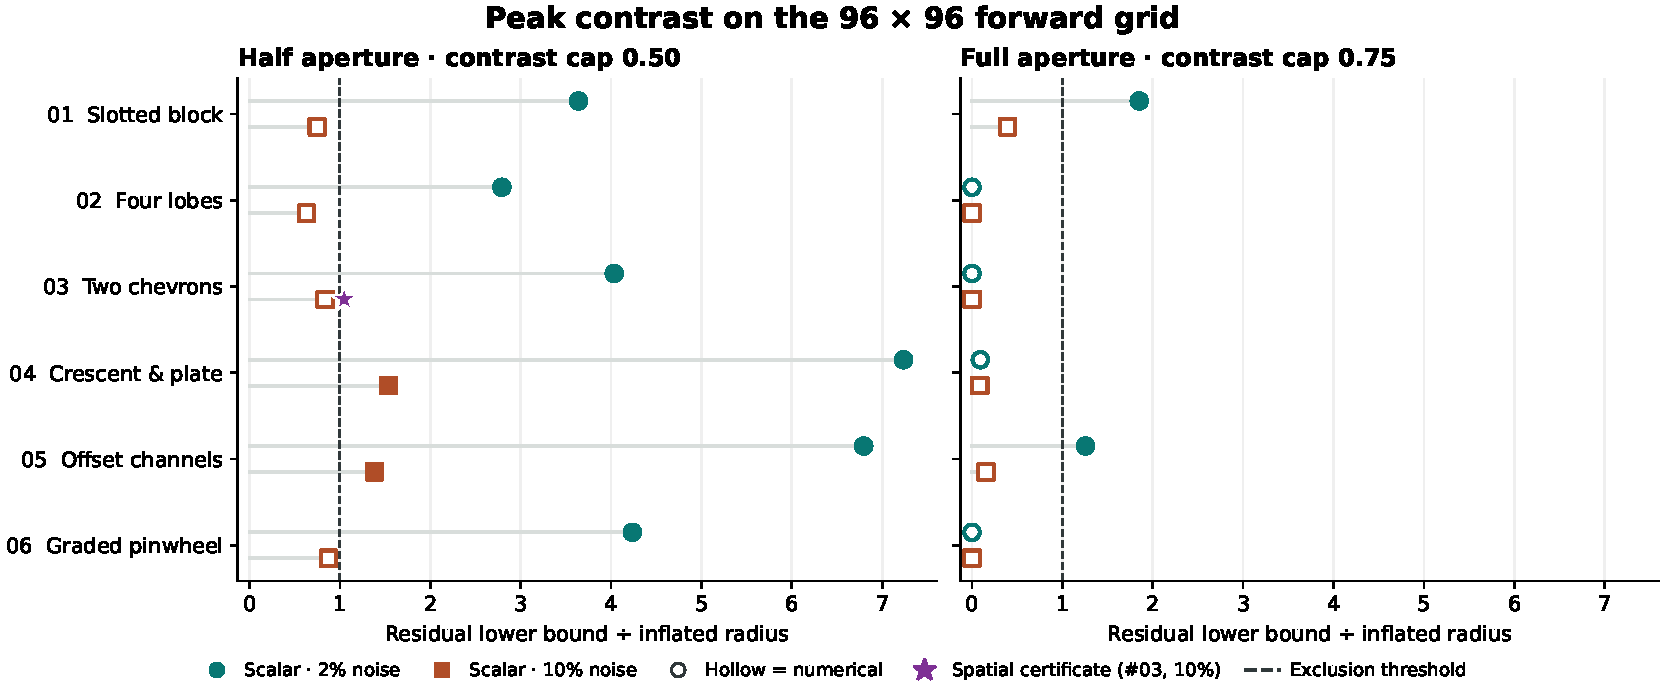
\includegraphics[width=.97\linewidth]{figure-01.pdf}
\caption{Measurements from the same six objects in two acquisition geometries. The half-ring panel tests peak contrast 0.5; the full-ring panel tests 0.75. A ratio above one excludes the entire indicated material box. The symbol key distinguishes the two original noise levels and the spatial proof for object 03. Hollow marks are numerical candidates and carry no exclusion claim.}\label{fig:apertures}
\end{figure}

\subsection{Full-ring noise curve and a third strict separation}
Table~\ref{tab:noise} gives the pre-specified full-ring thresholds at five levels of noise. The scalar multiplier search and the spatial search both use all source columns. The four-quadrant search allowed independent changes in the real and optical weights using \eqref{eq:gradient}. We separately reused two positive-definite sixteen-region profiles found on objects 01 and 05 at 2\%, keeping them fixed when applied across every shape and noise level. This distinguishes generalization of these particular profiles from retuning spatial weights on each data set. They produce no additional passing objects in the union. A negative outcome in these sweeps is a failure to obtain a certificate, not a physical material with the stated cap.

\begin{table}[tb]
\caption{Full ring, native grid. Counts are out of the same six materials. The final column lists every object proved to exceed 0.75. At each noise level, no tested weight yielded a positive exclusion at the higher thresholds 1, 1.25 and 1.5.}\label{tab:noise}
\centering\begin{tabular}{rccccc l}\toprule
 & $u=.5$ &\multicolumn{4}{c}{$u=.75$} & \\
Noise & Global & Global & 4 regions & Fixed 16 & Union & Objects in union\\ \midrule
0.5\% &6&3&3&2&3&01, 04, 05\\
1\%   &6&2&3&2&3&01, 04, 05\\
2\%   &6&2&2&2&2&01, 05\\
5\%   &6&0&0&0&0&---\\
10\%  &6&0&0&0&0&---\\ \bottomrule
\end{tabular}
\end{table}

A third strict separation occurs for object 04 at lower noise. At 1\% the padded radius is 0.0478678320. The best of 8,987 numerical global controls was replayed with a native \emph{upper} distance of 0.03667033; using the mean optical weight of the local design gave an upper distance of 0.03661415. These upper bounds apply to two specific global choices. With a uniform sector weight $10^{-4}$ and quadrant optical weights $(4,16,16,16)\times10^{-6}$, the native joint distance is at least 0.05077102. There are exactly four negative directions, with positive eigenvalues of $K/\mu$ at least 0.015625. In contrast, Theorem~\ref{th:two} constructs a zero-residual current for every globally constrained coherent source on this same observation. The finite global \emph{joint} search and the all-parameter global \emph{single-source} obstruction are logically separate comparisons. The overshoot is 0.00290318 absolute field units, or 6.1\% of the error radius. At 2\%, the four-quadrant result for this same object fails. A positive coarse-grid value at that condition would have reversed this conclusion.

\begin{figure}[tb]
\centering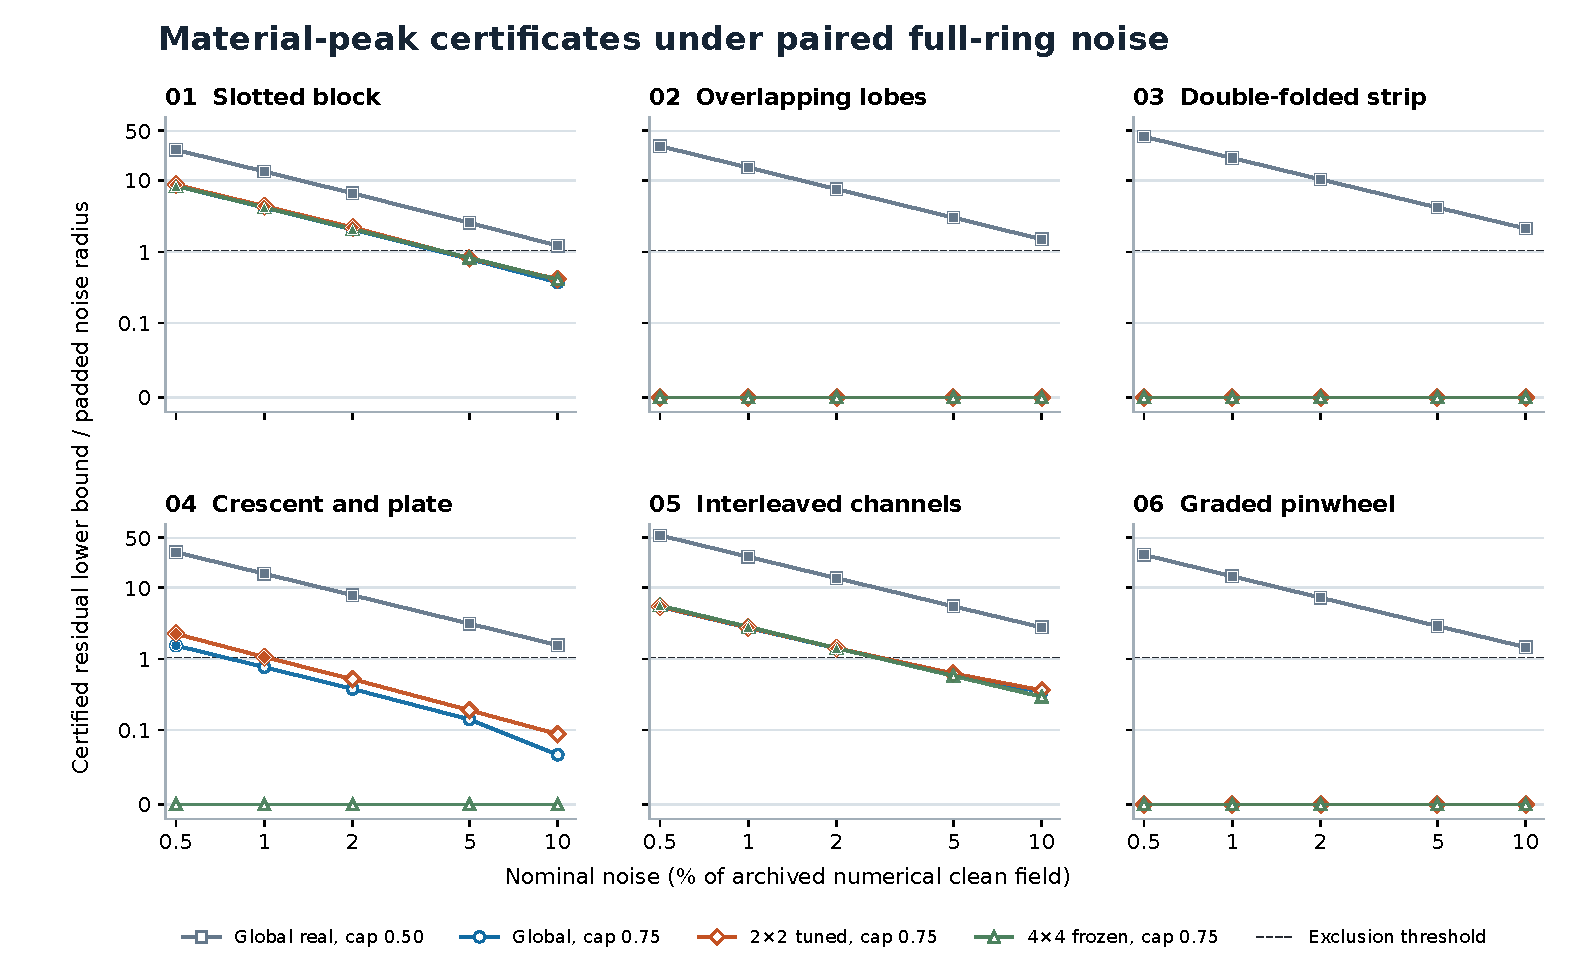
\includegraphics[width=\linewidth]{figure-02.pdf}
\caption{Full-ring noise series. Each panel follows a single shape along its fixed complex noise direction. A point above the horizontal unit line is a native interval exclusion. The low-contrast cap provides a reference. The spread across panels at 0.75 is larger than the change produced by several of the multiplier refinements. See Table~\ref{tab:noise} for the counts; a noise level does not create a new independent object.}\label{fig:noise}
\end{figure}

The global two-witness hypotheses and relative Slater inequalities were independently tested at $u=.75$ on all 30 public readings. The same dark vector has $k+10^4p\le-0.02088395$ and $p\ge5.3275\times10^{-7}$. At each of 0.5, 1, 2 and 5\%, all six views have a verified strictly feasible mean; at 10\% only 01 has the required verified signs for the chosen construction. Thus 25 views have the simultaneous single-source conclusion, including every full-ring joint exclusion at 0.75. In 01 and 05 at 2\%, the smallest eigenvalues of the negative optical Gram exceed 15.9286 and 5.3585. Those of the negative combined Gram exceed $1.3090\times10^5$ and $4.1228\times10^4$. Taking $\eps=2^{-40}$ gives positive Slater optical and sector slack and a lifted residual below $4.461\times10^{-7}$ in both cases, several orders below their error radii. The rank-one construction in Theorem~\ref{th:two} has exact zero residual. The other five 10\% cases have no conclusion from that fit proposal. The comparison therefore establishes multi-source/global-single strict separation on three distinct objects in total, across eight paired object--noise conditions.

\paragraph{Why higher caps failed.}
On the full ring the global weight screen at caps 1, 1.25 and 1.5 found minimum projected negative indices 13, 15 and 17 over 825 configurations per cap. The source dimension is ten. A data-independent interval obstruction strengthens this finite observation. For the four quadrants write $D_{\mu,b}=\mu w_b$ and $D_{\lambda,b}=\mu(t+\delta_b)$. Construct a ten-dimensional subspace of the receiver kernel by correcting proposed columns with $I-S^*(SS^*)^{-1}S$. On that subspace $K/\mu$ is multi-affine in $(u,w_b,t,\delta_b)$, since each product is between distinct parameters. For any parameter rectangle it is a convex combination of the vertex matrices. A shared ten-column witness negative definite at all vertices proves $\nu\ge10$ everywhere inside, for every $\mu>0$ and every reading.

For $1\le u\le1.5$, $0.875\le w_b\le1.125$, $-4\le t\le16$ and $|\delta_b|\le0.125$, a 1,024-vertex enclosure put the largest projected eigenvalue below $-0.03939$ at all vertices. For an alternative family, $0.5\le w_b\le1.5$, $t=0$, $|\delta_b|\le0.06$, the corresponding 512-vertex result was below $-0.03777$. All four sector and all four optical perturbations can vary independently. For each of the two fixed sixteen-region profiles, separate ten-direction certificates on the native grid likewise rule out a positive score at the three discrete higher caps. A trial common subspace for the wider quadrant box $|w_b-1|,|\delta_b|\le0.25$, $t\in[-4,16]$ failed at a vertex with upper eigenvalue about $+0.0673$. The claim does not cover arbitrary positive spatial multipliers. It explains why reducing observation noise, or optimizing the source once the source spectrum is empty, cannot rescue the proved multiplier families.

\subsection{Single-source spatial constraints and the price of a certificate}\label{sec:energy}
The strongest single-source comparison uses the same 20 receivers, ten original illuminations, complex observations, cap, and padded noise ball as the joint calculation. Both sides may select weights from the data and use the same spatial partition. A coherent combination $Ya$ uses the measured multistatic array; a physical acquisition of one preselected wave would give less information about which $a$ to choose. Thus the table tests processing of an identical array. It makes no assertion about how many transmitter firings an unknown target could save.

\begin{table}[tb]
\caption{Native full ring at 2\%, $u=.75$. Distances are in field units. Zero in the first two rows is an optimum for every unit complex mixture. Positive numbers in the lower rows are conservative lower bounds. The last line is the number of positive source eigenvalues at the certified sixteen-region profile.}\label{tab:compare}
\centering\begin{tabular}{@{}>{\raggedright\arraybackslash}p{.49\linewidth}rr@{}}\toprule
Method or quantity & 01 & 05\\ \midrule
Global coherent, simultaneous constraints &0&0\\
Four-region coherent SDP, simultaneous constraints &0&0\\
Shared constant weights, joint ($\nu=4$ in the proof) &0.16069878&0.11060787\\
Best verified global lower bound &0.16832983&0.11060787\\
Sixteen-region coherent, nonuniform profile &0.18967407&0.12452151\\
Joint at identical sixteen-region profile &0.18967407&0.12452151\\
Padded error radius &0.09096764&0.08802506\\
Positive source eigenvalues, same profile &1&1\\ \bottomrule
\end{tabular}
\end{table}

For the four-region comparator, four receiver-invisible vectors have an invertible matrix $(l_{bj})$ in \eqref{eq:localw}. Solving its four optical equations produces the $P_j$ in \eqref{eq:moment}. After outward rounding their smallest eigenvalues exceed $3.53\times10^{10}$ for object 01 and $5.83\times10^9$ for object 05. The largest local sector eigenvalues after the correction are below $-5.27\times10^8$ and $-8.70\times10^7$, respectively. The large covariance arises because weakly radiating currents can enter the moment matrix with large amplitudes while leaving the receiver residual unchanged. The comparison so far imposes the four pairs of regional balances alone. The constructed lifted moment has rank at most five, and the rank-one feasibility of the eight local constraints remains open. The joint certificate at constant weights is available in the same four-region family and strictly passes on both observations.

For sixteen regions, weights proposed using a block-polynomial trial space and ranked with the native operator lead to the opposite outcome. Section~\ref{sec:fourier} proves $K/\mu\succeq I/1024$ independently for each of the two chosen profiles. Each proof matrix has order 1,478. At these weights the source form is strictly negative on a verified nine-dimensional subspace; a certified positive leading Rayleigh quotient provides the complementary sign. The joint distance is enclosed in $[0.189674078449691,\,0.189674078449705]$ and $[0.124521510770564,\,0.124521510770574]$, respectively. Consequently the best coherent direction and joint trace have the same value for these profiles. The global multipliers are also contained in this spatial family. The experiments determine neither the overall optimum of the sixteen-region SDP across all weights nor the best possible joint bound. They do settle the original threshold question on these two objects: both competitors can exclude the cap of 0.75. Figure~\ref{fig:partition} illustrates how the answer depends on the strength of the single-source comparator.

\begin{figure}[tb]
\centering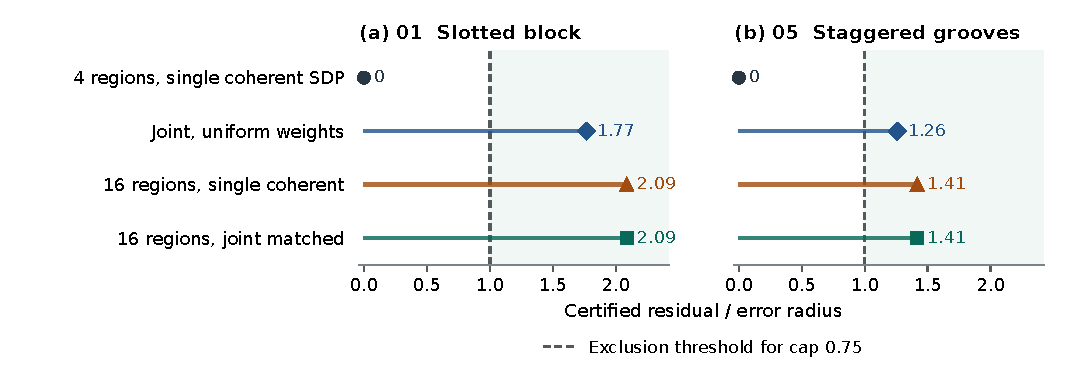
\includegraphics[width=.91\linewidth]{figure-03.pdf}
\caption{Original full-ring 2\% observations and the same padded noise balls for every comparison. Four-region single-source moments fit the readings exactly for every coherent source. Sixteen regions give an independently verified coherent exclusion in each object. Under those same weights, the joint spectrum has precisely one positive eigenvalue.}\label{fig:partition}
\end{figure}

\begin{table}[tb]
\caption{Wall time on the same Apple M4 for the two objects in Table~\ref{tab:compare}. Geometry is shared only where stated. The original global search covered 2,832 rows across several experiments and cannot be allocated exactly to these two objects. The uncertainty proof entails more work than one unverified numerical eigendecomposition.}\label{tab:cost}
\centering\begin{tabular}{@{}>{\raggedright\arraybackslash}p{.52\linewidth}r>{\raggedright\arraybackslash}p{.27\linewidth}@{}}\toprule
Operation & Seconds & Scope\\ \midrule
Global multi-source search, original complete scan &64.44& multiple apertures/caps\\
Fixed constant-weight joint inertia proof &6.61& one shared 645-order system\\
Four-region single-source zero optimum, construction and proof &6.95& both objects, 1.69 s shared setup\\
Sixteen-region symmetric trial search &66.29& 84 trials, missed object 05\\
Nonuniform candidate search and native ranking &22.49& both objects\\
Verified sixteen-region coherent distances &69.44& both, 34.75 and 34.42 s per object\\
Joint source spectrum with the two proofs reused &6.09& both objects, warm\\
Cross-application to all thirty paired observations &20.50& both profiles, warm\\ \bottomrule
\end{tabular}
\end{table}

The nonuniform path cost 91.93 s for both objects from candidate search through verification, or 158.22 s when the preceding unsuccessful symmetric search is included. The two full coherent proofs use four interval FFT columns in total; the initial numerical searches use many more. The compact constant-weight proof could be reused across the two objects, while the data-specific sixteen-region choices required separate state proofs. No physical material-reconstruction solve is hidden in these times. Krylov iterations, FFT applications, trial screening, and interval verification are recorded separately. These times describe the observed cost of the reported bounds.

\paragraph{Current energy and the four-region comparison.}
For one unit coherent direction $a$, take any physical current $j$ satisfying the cap and $\|Sj-Ya\|_2\le r$. Given weights for which $K\succ0$, choose $0<\tau<\lambda_{\min}(K)$ and set $K_\tau=K-\tau I$ and $H_\tau=Y^*Y-L^*K_\tau^{-1}L$. Completing the scalar quadratic in $j$ using $K_\tau$ gives
\begin{equation}
 \|Sj-Ya\|_2^2\ \ge\ \tau\|j\|_2^2+a^*H_\tau a .
 \label{eq:energybound}
\end{equation}
Thus a verified lower bound $\ell_\tau\le\lambda_{\min}(H_\tau)$ gives $\|j\|_2^2\le(r^2-\ell_\tau)/\tau$ uniformly over the unit source sphere. All energies use the saved cell coordinates. Area weighting rescales both the bounds and the moments by the cell area.

A second bound applies to the whole material box without a receiver tolerance. Approximate $R=\Imag G$ by the Gram $TT^*$ of 64 angular plane-wave columns and write $S^*=TA+F$. For $\chi>0$,
\[
 S^*S\preceq (1+\chi)\|A\|_2^2 TT^*+(1+\chi^{-1})\|F\|_2^2 I.
\]
An enclosure of $TT^*-R$ and upper bounds on the two norms give $S^*S\preceq\gamma R+\eta I$. For this ring take $\gamma=1/128$ and $\eta<5.14\times10^{-10}$. Since $\eta<\mu/1024$, the verified sixteen-region floor gives $K_{\rm p}:=K-S^*S+\gamma R\succ0$. The added term arises from increasing the global optical weight by $\gamma$. The new linear coefficient is $Z_{\rm p}B$ with $Z_{\rm p}=Z+\mathrm i\gamma I/2$. Completing the physical quadratic with $K_{\rm p}-\tau I\succ0$ gives a bound by $\lambda_{\max}(B^*Z_{\rm p}^*(K_{\rm p}-\tau I)^{-1}Z_{\rm p}B)/\tau$, with no data term.

We use the frozen sixteen-region weight fields and tighten their verified gap to $K/\mu\succeq(3/256)I$. The whole-box bound is $2{,}340{,}476$ for both observations. The bounds conditional on the coherent error balls are $4{,}982{,}633$ for object 01 and $1{,}035{,}001$ for object 05. Either bound applies inside its corresponding error ball, so one can use the smaller.

In the four-region semidefinite problem let $X_a$ be the current--current block of the lifted matrix $W$. The energy constraint is $\tr X_a\le C_{\rm en}$, where $C_{\rm en}=(r^2-\ell_\tau)/\tau$ and $\tr W=1+\tr X_a$. A uniform certificate of zero optimal discrepancy follows if the matrices in \eqref{eq:moment} also satisfy
\begin{equation}
 X^*X+\sum_j\|v_j\|_2^2P_j\preceq C_{\rm en} I_s .
 \label{eq:momentenergy}
\end{equation}
Indeed the trace of the current moment for $a$ is the quadratic form of the left-hand side on $a$.

We construct a new receiver-exact mean and eight dark vectors for each observation. On the native grid, outward rounding verifies positive moment weights, strict sector inequalities and a uniform energy below 8,500 for object 01 and 7,000 for object 05. The optical equalities hold by construction and the moments have rank at most nine. The generating materials have peaks above $0.75$. For offline comparison their largest coherent energies $\|J_{\rm ref}\|_2^2$ are approximately 66,192.79 and 31,647.96. The two witness upper bounds are less than $13\%$ and $23\%$ of those reference energies.

A material constant on $12\times12$ regions within the $0.75$ box has physical energy above 8,886.62 for a fixed unit coherent input, as verified by an interval forward check using no observed fields. Any scalar energy cap valid for the whole material box and every unit input must therefore exceed this value. Both moment witnesses fit under every such cap. The individual error-ball caps are justified separately by \eqref{eq:energybound}.

For each object the four-region SDP has exactly zero optimal distance for every unit coherent input at each energy cap in the sweep, namely $10\|J_{\rm ref}\|_2^2$, $100\|J_{\rm ref}\|_2^2$, $10^6$, $10^8$, the whole-box cap, the error-ball cap, and $+\infty$. Once a witness fits at a given cap it fits at every larger cap, so this conclusion follows from the same interval proof across the sweep. The fixed global-weight joint bounds remain 0.16069878 and 0.11060787, above their padded error radii of 0.09096764 and 0.08802506. Thus the joint exclusion persists against this energy-constrained four-region comparator.

At an artificial cap of 100, a receiver-only relaxation gives lower bounds of 0.9730 and 1.0280 for the best coherent distances. The exact transition to a positive optimum remains open.

Across both objects, tightening the spectral gaps and verifying the error-ball bounds took 283.57 s including setup. The whole-box proof took another 4.30 s using one of those gaps. The final moment construction and proof took 3.59 and 7.09 s, with 36 interval Green applications in the proof. The physical check and its controls took 1.19 s. These wall times exclude separate search trials and offline reference solves.

\subsection{A data check on an underfitted reconstruction}
We tested what a peak certificate contributes alongside a standard forward residual check. A conventional nonnegative Tikhonov Gauss--Newton reconstruction starts from zero contrast. Its ridge is one tenth of the largest squared singular value of the background Jacobian. Each proposed step uses the full Jacobian and a full-wave acceptance test. Neither the parameter nor the stopping rule uses the reference image. The same normalized rule is applied to both examples. It is deliberately a test of an underfitted reconstruction, not a comparison with an optimally tuned imaging method.

On an archived 576-cell ring, the seventh accepted update met the objective stopping rule at peak 4.75615. A direct interval forward solve gave a residual in $[0.9341373929,0.9341373930]$, far above the noise radius 0.01051719. An ordinary residual check thus rejects this specific reconstruction. With the \emph{same} readings, a peak-wide lower bound of 0.01469495 excludes every nonnegative material whose peak is at most 5. This adds a property of the entire feasible set. An offline check places the generating material, peak 12, within the ball. On the native $96^2$ half-ring slotted block at 2\%, the first two iterates have peaks 0.22816 and 0.36992, below the excluded cap of 0.5. The third crosses it; the prescribed twelve-update endpoint reaches 0.80150. Its residual 3.46297 still exceeds the radius 0.10133. This second endpoint does not provide another below-cap terminal case. The diagnostic can be applied before or after reconstruction without iterating on the unknown material.

\begin{figure}[tb]
\centering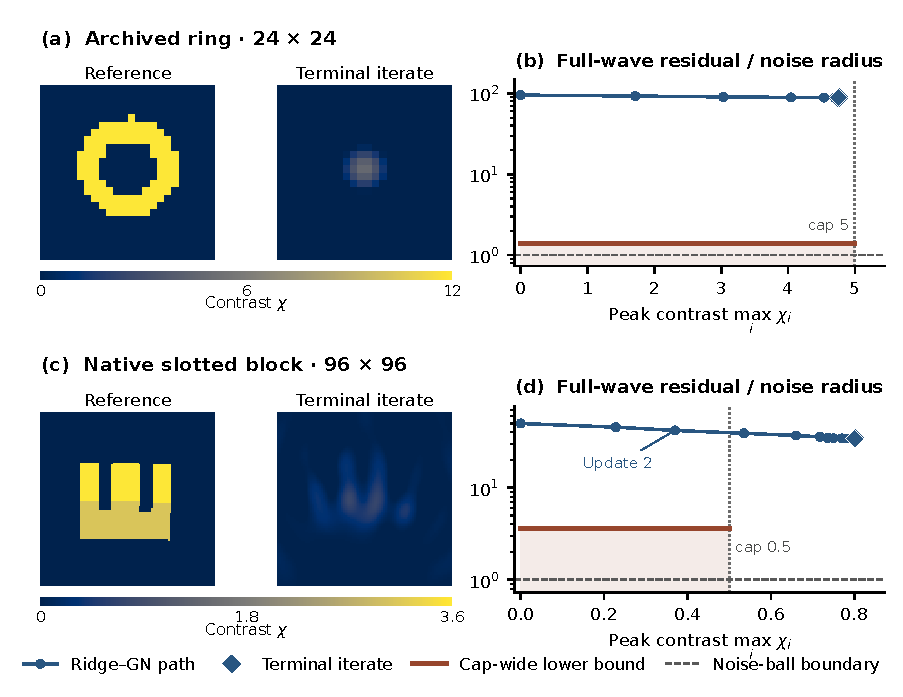
\includegraphics[width=.96\linewidth]{figure-04.pdf}
\caption{Reference materials, terminal Gauss--Newton reconstructions and accepted iteration paths. The peak test rules out every material in the indicated lower peak range. The pointwise residual check tests each displayed iterate individually. Only the 576-cell object terminates below its certified cap under the fixed rule; the native slotted block crosses the cap at update three.}\label{fig:check}
\end{figure}

\subsection{Regional localization, two frequencies and measured data}
A separate archived experiment tested sixteen regions in seven views of six high-contrast $32^2$ objects. At both $U_{\max}=20$ and the tighter conditional prior $U_{\max}=4$, none of the 112 region--view pairs could be certified by the tested family, even when the region in question was taken to be empty. Proposition~\ref{prop:exterior} explains the common failure. With cap 20, the native exterior contained at least 116 negative directions for the twenty-source group and at least 106 for the ten-source group. With background cap 4 the lower bounds were 24 and 14, still larger than their respective source counts. These are certified results for the archived operator, audited range of exterior multipliers and unrestricted tested interior weights. No new region experiment was used to enlarge the sample. The ability to exclude a small \emph{global} peak provides no implication that a particular block must contain a high contrast.

An existing comparison also tested two frequencies on the six objects with the same half array at 400 and 500 MHz. Each frequency used its own Green, receiver and incident field. With a shared, nondispersive real material, the block-diagonal stack repeats the same $M$ at each frequency: a Hermitian weight mixing frequencies at a single pixel commutes with this repeated material. This permits the same derivation as \eqref{eq:sector}--\eqref{eq:bound}. Alternatively one can certify each frequency separately and add squared lower distances. At $u=.5$ and 2\% noise the independent bounds passed three cases and the tested mixed stack passed none. At 10\% both arms passed none. These results were for the inverse-grid operators against the nominal data radius. Adding even the per-object observed coarse-proxy discrepancy removed the three passes. The two arms received identical fields, and the mixed method had to pay a common negative-index penalty. The experiment supplies neither a native-grid multifrequency peak exclusion nor a reason to expect stacking always to improve the proof.

We finally retain a measured-field test using three dielectric targets in the 2005 Institut Fresnel free-space database \cite{fresnel}. Scattered complex fields were obtained from the measured total and incident fields, at 4, 6 and 8 GHz. Each transmitter had 241 valid receiver angles. The internal and external two-cylinder objects had eight illuminations and the twin object had eighteen. There was no common receiver row over every source in a full acquisition. Disjoint source groups with common measured receivers were therefore retained as described in Section~\ref{sec:joint}. The forward comparisons used a $60^2$ square grid. Neither target identity nor template contrast was used in constructing the certificates.

At a cap of 0.5 none of the nine object--frequency cases exceeded the held-out calibration scale. To quantify the margin, consider the twin target. At 4 GHz a six-source group with negative index five contributed to a positive bound of 0.45358\% of the data norm at $u=.5$, against an empirical additive scale of 8.88355\%. At 6 and 8 GHz the positive indefinite bounds at $u=.25$ were 1.922\% and 3.409\%, short of the corresponding error scales by 35.32 and 45.07 percentage points. A simpler real-sector bound at 4 GHz and $u=.25$ reached 28.515\%. With a putative gain cap of 10.41\% and additive cap of 8.884\%, \eqref{eq:budget} leaves 6.98\% of $\|Y\|_F$ for the unknown physical discrepancy. The held-out empty-scene RMS is not a guaranteed loaded-scene error radius. Hence even this last, positive margin remains conditional. No unconditional lower dielectric bound is claimed for these measured targets.

\subsection{Transfer to archived materials and to another laboratory}
We applied the frozen tests to all eligible materials in two simulation archives. Selection used the acquisition metadata. These objects had been scored for other inversion methods; they had not served to adjust the transferred profiles. Truth entered only after sealing the data-based results. Table~\ref{tab:transfer} reports whole-box exclusions. The second array is illustrated in figure~\ref{fig:transfer-array}. The two arrays have different noise levels, source fields and receivers. Their threshold difference cannot be assigned to a change in the number of ports alone.

\begin{table}[tbp]
\centering\small
\caption{Two frozen-profile transfers. Each denominator counts materials, with one original noisy observation per material. The coherent input is optimized for the same profile and is tested against the same deterministic error radius.}
\label{tab:transfer}
\begin{tabular}{lrrrr}
\toprule
Acquisition & Cap $u$ & Objects & Joint & Coherent\\
\midrule
$96^2$, 10 transmit, 20 receive, 10\% & 0.50 & 22 & 22 & 20\\
Same, five inherited profiles & 0.75 & 22 & 0 & 0\\
$24^2$, 12 transmit, 48 receive, 1\% & 5.00 & 7 & 5 & 0\\
\bottomrule
\end{tabular}
\end{table}

For the 22-object transfer, two materials previously examined in the optical study were removed from the 24-object archive. The input was the original full-ring field. At $u=.75$ the most favourable upper endpoint, over 110 object--profile pairs, was only 0.1682 times its radius. This is an upper bound on the specified certificate, not on the distance to the material box. The known full-resolution contrasts ranged from 2.51 to 4.06. All 22 generating media were verified inside the declared balls $\delta+10^{-6}\norm{Y}_F$; 11 lay just outside the original sampled radius when evaluated on the stored operator. The six-profile replay took 63.2 seconds in total. Among 176 saved reconstruction outputs on the matching observations, five from two objects assigned a peak of at most 0.00570. Their piecewise-constant extensions to the native mesh preserve that peak, so the data contradict all five. A coarse cell average alone allows unresolved fine-scale peaks.

The second acquisition exactly reproduced the stored $G,B,S$ of the earlier ring in section~\ref{sec:exp}. With the original real-sector weight $\mu=.001$ and $\lambda=0$, the verified negative index was four. Cases 03, 06, 12, 15 and 21 excluded $u=5$ by factors of 5.12 to 10.77 over their original radii. All seven reference media were inside their respective noise balls. Case 09 had peak 16.25 yet the larger multiplier search certified only $u=3$. Case 18 had peak 4.28 and could not validly exclude $u=5$. At $u=4$ five coherent tests on the preselected grid matched the joint count. At $u=5$ no tested coherent profile crossed. Extending the strict global single-source separation theorem to these seven observations remains open. All 77 archived same-grid reconstruction peaks exceeded the corresponding certified caps.

\begin{figure}[tbp]
\centering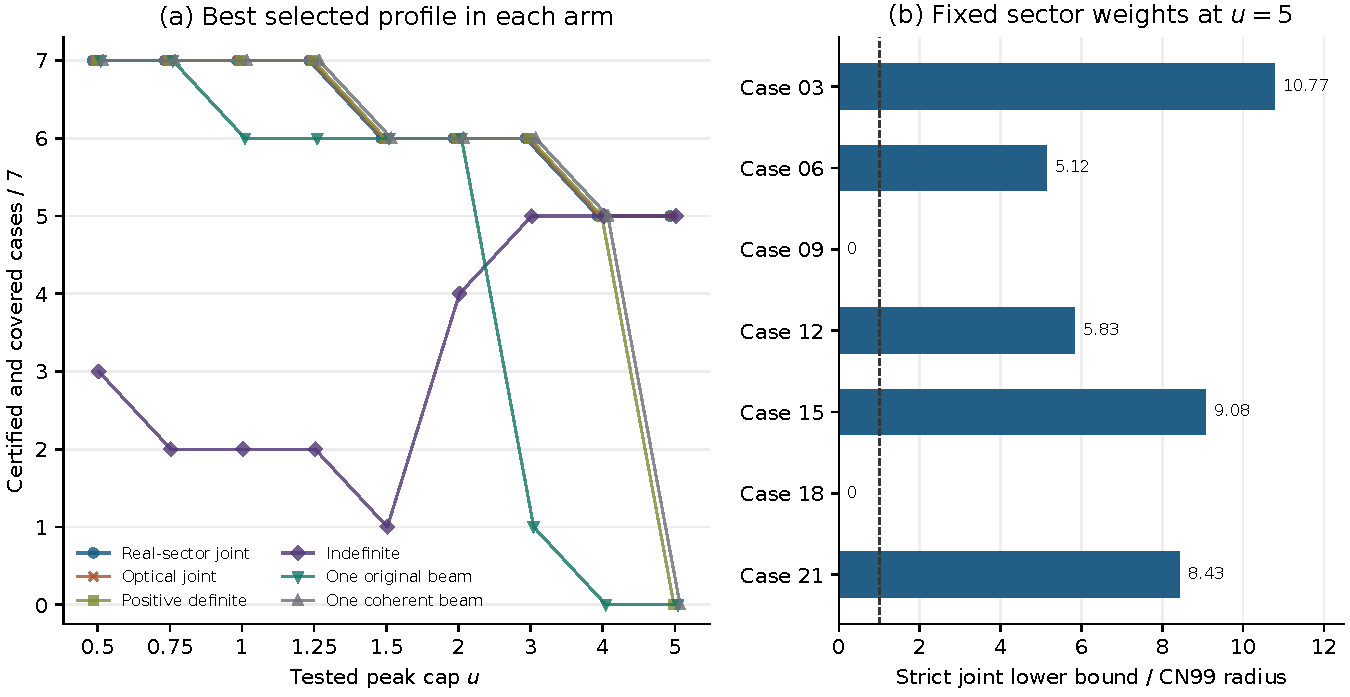
\includegraphics[width=.98\linewidth]{figure-05.pdf}
\caption{Twelve transmitters and 48 receivers, seven archived objects at 1\% noise. The left panel counts exclusions for each tested cap and multiplier family. The right panel gives the joint distance bound divided by the original noise radius for each object with fixed global weights at $u=5$. A ratio above one rules out every material with peak at most five. Object 09 had peak 16.25 and remained undecided at this cap.}\label{fig:transfer-array}
\end{figure}

For an independent measured acquisition, we used all four dielectric configurations and all seven frequencies of the July 2010 Manitoba tomography dataset, from 3 to 6 GHz \cite{manitoba}. Two complementary, reciprocal $12\times12$ port blocks provide 288 of the 552 acquired directed channels. We subtracted the first empty chamber and calibrated using the larger metal cylinder. The second empty chamber and the smaller cylinder provided independent checks. A $40^2$ two-dimensional port model supplied the rigorous discrete bounds. The two blank choices crossed with the two metal standards give four estimates $Y_j$ of the complex field for each target. If $d$ is a proved lower distance at the primary estimate $Y_0$, then every field in their convex hull has distance at least $(d-\max_j\norm{Y_j-Y_0}_F)_+$ to the same below-cap model set.

Figure~\ref{fig:cal-headroom} reports the remaining error allowance in units of the primary field. With passive-compatible multipliers this remaining distance was positive on 20, 5, 3 and 1 of the 28 observations at caps .25, .50, .75 and 1, respectively. Each object contributed seven frequencies. Interchanging source and receiver identified an antisymmetric component of 0.62--5.98\% of the primary norm. Replaying the same profiles on the symmetric fields, with the four calibrations projected in the same way, gave the same passing observations. For the E-shaped phantom at 3.5 GHz, the cap .50 still left 1.358\% of the primary field norm for further discrepancy. The large nylon cylinder at 3 GHz left 4.018\% at cap 1. For a passive lossy contrast $\chi=x+iy$ the cap concerns $x+y^2/x$ for $x>0$; a claim about $x$ alone requires a material loss bound. Neither the four calibrated fields nor the mesh comparison bounds the loaded-target model error.

\begin{figure}[tbp]
\centering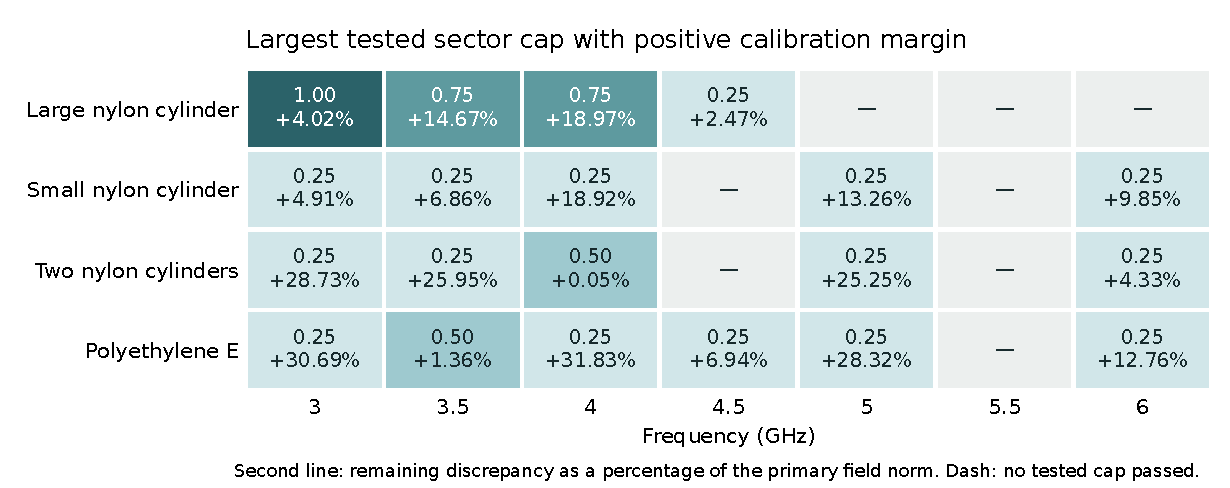
\includegraphics[width=.98\linewidth]{figure-06.pdf}
\caption{Remaining allowance for target-dependent error in Manitoba measurements, relative to the norm of the primary calibrated field. Four combinations of two empty-chamber readings and two metal references define the calibration set. Positive entries leave room for further error at the indicated passive material cap. For the nylon pair at 4~GHz, only 0.053\% remains at $u=.5$. The two-dimensional model error for the loaded chamber is unknown.}\label{fig:cal-headroom}
\end{figure}

\FloatBarrier
\section{Discussion and limitations}\label{sec:discuss}

\subsection{What is identifiable in this experiment?}
For a specified acquisition, model and error ball, the output is a strict lower bound on the largest real, nonnegative contrast. It applies to arbitrary configurations of all cells in that model. The location of the maximizing cell, the number of defects and their shape need not be identifiable. The gap to the actual peaks illustrates this distinction: the six reference peaks exceed 3.3, whereas the highest native cap excluded on these same full-ring objects is 0.75. A larger certified cap on a different ring cannot be transferred by counting more pixels. A proposed interpretation of the readings can be contradicted independently of a reconstruction algorithm and its termination rule.

Two effects contribute to the result. A partial receiver array may miss radiated power. An optical equality can then disqualify currents that satisfy the real-sector inequality and fit the readings. Separately, a shared array of incident fields imposes a deterministic cross-illumination Gram. A small number of negative state directions need not be able to mask its positive residual in all source directions at once. These effects require different controls. The half-ring ablation changes the optical constraint at fixed data. The global two-witness construction changes the quantifier over sources while enforcing both constraints simultaneously. The four-region moments and sixteen-region coherent certificate expose the role of spatial information under the same data budget.

Four regional balances allow receiver-invisible covariance to offset the optical and sector forms of a receiver-exact mean. The new witnesses in Section~\ref{sec:energy} preserve this mechanism under every uniform energy cap valid on the entire material box and under both certified data-conditioned caps. With sixteen regions, two verified weight fields make the state quadratic positive and leave a single positive source eigenvalue. A coherent projection then carries the entire fixed-weight bound. For the two sixteen-region profiles the largest diagonal entries of $H_Y$ are bounded above by $-0.7450$ and $-0.2621$ for 01 and 05. Each individual original illumination therefore has a zero nonnegative score at those fixed weights. A wavelength-dependent block-size law, a physical resonance inside one subregion, and a unique propagating channel of the actual object would be stronger conclusions. We establish the signs of two weighted operators and the number of positive directions of their data-dependent source matrices. The physical scattering matrix can have higher rank.

Finite-data uniqueness depends on both the experiment and the prior. Alberti and Santacesaria prove finite-measurement recovery under explicit restrictions on the coefficient space \cite{alberti19,alberti21}. Kuo and Novikov show how changing from the full fixed-energy far field to one incident direction alters uniqueness even for a collection of point scatterers \cite{kuo_novikov}. Sparse-array recovery for localized Foldy--Lax scatterers uses support and coherence assumptions \cite{chai}; completion of a scattering $T$ matrix uses consistency between the interaction and the measured data \cite{levinson}. The present peak test admits all cell arrangements in the contrast box. It returns information about their common peak constraint when their locations remain unresolved.

\subsection{Relation to prior results and computation}
The power identities follow from a shared, local constitutive law. Photonic bounds for convex field objectives, simultaneous real and reactive power, subdomain restrictions and cross-excitation consistency already address important parts of this structure \cite{trivedi,moleskyglobal,moleskylocal,shim}. The completion and negative-index count have a matrix-analytic foundation \cite{tian}. Specifying a measured residual and an error radius alone would give only a change of objective in those frameworks. Our affirmative result concerns two conclusions in the \emph{same} incomplete-aperture experiment: a current fitting each coherent datum and satisfying both global laws, and a joint bound contradicting every below-cap material. The distinction persists against a four-region SDP with a certified energy cap for two observations. Sixteen regions give counterexamples to extending that interpretation at the same threshold. The continuum support theorem using monotonicity modulo finitely many directions \cite{albicker} addresses a different inverse statement; it does not predict the residual margins or the finite-source SDP comparison computed here.

A complementary approach is to describe the set of nonlinear solutions. Everett and Vasco trace multiple solutions in finite-dimensional geophysical inversions \cite{everett96,vasco,everett26}. Set inversion by interval analysis can enclose a bounded-error parameter set by successively subdividing the prior box \cite{sivia}. Here a single positive residual margin eliminates a complete contrast box without resolving its boundary in parameter space. An inconclusive margin leaves that box undecided. Neither the location nor the number of inverse solutions follows from this test.

The Fourier step reduces the dimension of the proof matrix. For $p$ receive channels and $k$ retained Fourier modes the compact order is $p+k$ for a constant multiplier and at most $p+2k$ in the two-field construction. Dense factorization costs order $(p+2k)^3$ arithmetic operations, with a precision dependence in the interval work. Reading the full symbol and applying the native operator remain necessary. The number $k$ is governed by a valid omitted-spectrum floor. Trial dimensions, candidate counts, Krylov iterations and unsuccessful searches for a spectral gap incur additional costs. A single compact factorization characterizes a reusable proof for one fixed geometry and profile. Establishing mesh-independent performance or end-to-end polynomial complexity over arbitrary spatial profiles would require new estimates.

\subsection{Boundary of transfer}
All new positive thresholds for the full-ring comparison concern the exact \emph{stored} finite-dimensional scalar TM propagator, port maps and data. Subsequent numerical arithmetic is enclosed. Continuum kernel quadrature, a uniform material-to-continuum error bound, and physical calibration of an unknown loaded apparatus are distinct sources of uncertainty. Transferring the claim would require a physically justified bound in \eqref{eq:budget}. Receiver masks, polarization, aperture normalization and added channels can change the effective radiation and surviving source directions. In three dimensions the tensor constitutive law and dyadic radiation operator require separate analysis. With absorption both the sector prior and allowed optical multiplier signs change.

The six original shapes and their paired noise levels test sensitivity. The two archival transfers broaden the set of objects and retain their original acquisition and noise differences. None of these comparisons provides a population success probability or a validation of adaptive frequency selection. Even at 0.5\% noise the six-shape study yields no full-ring cap of 1. The negative-subspace theorem identifies continuous families in which reducing noise cannot help. On measured data, the allowable discrepancy can instead be read directly from the remaining margin. Both outcomes specify which material statements the measurements and their error model support.

\subsection*{Data and code availability}
The research archive contains the fixed synthetic operators and noisy fields, proof scripts, enclosed distances, timings, unsuccessful searches and the data underlying the figures. For the seven-object transfer the public archive provides every input needed to reproduce the online certificates and the offline feasibility statistics; the original reference images remain with the originating project. The two measured acquisitions are available from the originating laboratories \cite{fresnel,manitoba}. The archive includes the masks, calibration analysis and derived results used here. An anonymised copy of the numerical inputs and results can be supplied to the editors for review.

\section*{Acknowledgements}
\paragraph{Use of generative AI tools.} OpenAI Codex assisted with the mathematical arguments, numerical implementation, literature retrieval and manuscript drafting. Google Gemini examined the saved numerical evidence and suggested controls for the spatial partitions and for reciprocity in the calibrated chamber fields. The figures use the recorded data. Section~\ref{sec:exp} and Appendix~\ref{app:replay} describe how the numerical claims were checked. Responsibility for the analysis, interpretation and text rests with the authors.

\appendix
\section{Reading and replaying a certificate}\label{app:replay}

The native replay reads the padded Green symbol, the $20\times9216$ receiver, the $9216\times10$ incident fields, one complex reading and its radius.

\paragraph{Zero residual.}
Project the four proposed currents into $\ker S$ and solve the optical system in \eqref{eq:moment}. Verify its nonsingularity, positive definiteness of each $P_j$ and strict negativity of each local sector. The defining equations then give exact optical balance and zero receiver residual without assembling the $9217\times9217$ lifted matrix.

\paragraph{Positive distance.}
Enclose the compact inertia in complex ball arithmetic \cite{arb} and bound the full-grid defect of the numerical stationary point. In the positive definite coherent test, normalize a proposed source vector using its enclosed norm. The matched joint replay bounds the remaining nine directions above by zero. For an indefinite state form, sum the surviving positive source eigenvalues and compare the square root with the upper noise radius.

\paragraph{Current energy.}
Evaluate the shifted quadratic at its proposed stationary point and bound the correction by the squared Frobenius norm of the stationary defect divided by the verified spectral floor. For the constrained moment witness, enclose the source matrix in \eqref{eq:momentenergy} after correcting the fitted mean and the dark vectors to satisfy the receiver equations exactly.

\paragraph{Inconclusive tests.}
An upper bound below the radius rejects a specified multiplier. A ten-dimensional negative subspace forces zero throughout the audited high-cap families. Failure to construct a single-source feasible witness leaves feasibility open.

\begin{table}[tb]
\caption{Wall and process CPU seconds for the full-ring noise experiment. At $u=.75$ the global and four-region costs each include 45 inconclusive evaluations and the subsequent resolution of the 15 affected observations. Concurrent operations are timed separately. Fixed state-proof construction is listed separately in Table~\ref{tab:cost}.}\label{tab:replay}
\centering\begin{tabular}{lrr}\toprule
Operation & Wall (s) & CPU (s)\\ \midrule
Shared proposal search &12.79&12.73\\
Global native proof, $u=.5$ &49.52&49.97\\
Global native batch, $u=.75$ &213.88&211.86\\
Global refinement of 15 observations &20.20&19.98\\
Four-region native batch, $u=.75$ &316.14&312.89\\
Four-region refinement of 15 observations &42.40&42.50\\
Fixed sixteen-region profiles, thirty views &20.50&21.36\\
Three higher caps, same fixed profiles &14.59&14.88\\
Object 04, dense global control including search &59.53&58.62\\ \bottomrule
\end{tabular}
\end{table}

\paragraph{Cost and rounding.}
The code uses the full $192\times192$ zero-padded synthetic Green spectrum. Numerical search, interval evaluation and offline reference feasibility are timed separately. The enlarged noise ball is fixed before deciding whether a material cap passes. Table~\ref{tab:replay} gives the cost of the complete paired comparison. The two continuous high-cap multiplier rectangles cost an additional 8.64 s for trial subspaces and 6.50 s for the strict verification. The global simultaneous-fit and Slater replay took about 26 s over thirty data sets. 

\FloatBarrier
\begingroup
\small
\begin{thebibliography}{99}\setlength{\itemsep}{0pt}\setlength{\parsep}{0pt}
\bibitem{colton} Colton D and Kress R 2019 \emph{Inverse Acoustic and Electromagnetic Scattering Theory} 4th edn (Cham: Springer) \href{https://doi.org/10.1007/978-3-030-30351-8}{doi:10.1007/978-3-030-30351-8}
\bibitem{chenbook} Chen X 2018 \emph{Computational Methods for Electromagnetic Inverse Scattering} (Singapore: Wiley) \href{https://doi.org/10.1002/9781119311997}{doi:10.1002/9781119311997}
\bibitem{csi} van den Berg P M and Kleinman R E 1997 A contrast source inversion method \emph{Inverse Problems} \href{https://doi.org/10.1088/0266-5611/13/6/013}{\textbf{13} 1607--1620}
\bibitem{nie} Zhong Y, Lambert M, Lesselier D and Chen X 2016 A new integral equation method to solve highly nonlinear inverse scattering problems \emph{IEEE Trans. Antennas Propag.} \href{https://doi.org/10.1109/TAP.2016.2535492}{\textbf{64} 1788--1799}
\bibitem{cie} Zhong Y and Xu K 2019 Contraction integral equation for three-dimensional electromagnetic inverse scattering problems \emph{J. Imaging} \href{https://doi.org/10.3390/jimaging5020027}{\textbf{5} 27}
\bibitem{chen} Chen X 2010 Subspace-based optimization method for solving inverse-scattering problems \emph{IEEE Trans. Geosci. Remote Sens.} \href{https://doi.org/10.1109/TGRS.2009.2025122}{\textbf{48} 42--49}
\bibitem{zhong} Zhong Y and Chen X 2009 Twofold subspace-based optimization method for solving inverse scattering problems \emph{Inverse Problems} \href{https://doi.org/10.1088/0266-5611/25/8/085003}{\textbf{25} 085003}
\bibitem{cakoni_book}
Cakoni F, Colton D and Haddar H 2023 \emph{Inverse Scattering Theory and Transmission Eigenvalues} 2nd edn, CBMS-NSF Regional Conference Series in Applied Mathematics vol 98 (Philadelphia, PA: SIAM) \href{https://doi.org/10.1137/1.9781611977424}{doi:10.1137/1.9781611977424}
\bibitem{cakoni_vogelius}
Cakoni F and Vogelius M S 2023 Singularities almost always scatter: regularity results for non-scattering inhomogeneities \emph{Commun. Pure Appl. Math.} \href{https://doi.org/10.1002/cpa.22117}{\textbf{76} 4022--47}
\bibitem{trivedi} Trivedi R, Angeris G, Su L, Boyd S, Fan S and Vu\v{c}kovi\'{c} J 2020 Bounds for scattering from absorptionless electromagnetic structures \emph{Phys. Rev. Applied} \href{https://doi.org/10.1103/PhysRevApplied.14.014025}{\textbf{14} 014025}
\bibitem{angeris19} Angeris G, Vu\v{c}kovi\'{c} J and Boyd S P 2019 Computational bounds for photonic design \emph{ACS Photonics} \href{https://doi.org/10.1021/acsphotonics.9b00154}{\textbf{6} 1232--1239}
\bibitem{moleskyglobal} Molesky S, Chao P, Jin W and Rodriguez A W 2020 Global $\mathbb{T}$ operator bounds on electromagnetic scattering: upper bounds on far-field cross sections \emph{Phys. Rev. Research} \href{https://doi.org/10.1103/PhysRevResearch.2.033172}{\textbf{2} 033172}
\bibitem{moleskylocal} Molesky S, Chao P and Rodriguez A W 2020 Hierarchical mean-field $\mathbb{T}$ operator bounds on electromagnetic scattering: upper bounds on near-field radiative Purcell enhancement \emph{Phys. Rev. Research} \href{https://doi.org/10.1103/PhysRevResearch.2.043398}{\textbf{2} 043398}
\bibitem{kuang} Kuang Z and Miller O D 2020 Computational bounds to light--matter interactions via local conservation laws \emph{Phys. Rev. Lett.} \href{https://doi.org/10.1103/PhysRevLett.125.263607}{\textbf{125} 263607}
\bibitem{angeris} Angeris G, Vu\v{c}kovi\'{c} J and Boyd S 2021 Heuristic methods and performance bounds for photonic design \emph{Opt. Express} \href{https://doi.org/10.1364/OE.415052}{\textbf{29} 2827--2854}
\bibitem{shim} Shim H, Kuang Z, Lin Z and Miller O D 2024 Fundamental limits to multi-functional and tunable nanophotonic response \emph{Nanophotonics} \href{https://doi.org/10.1515/nanoph-2023-0630}{\textbf{13} 2107--2116}
\bibitem{tian} Tian Y 2013 Closed-form formulas for calculating the extremal ranks and inertias of a quadratic matrix-valued function and their applications \href{https://arxiv.org/abs/1301.2567v1}{arXiv:1301.2567v1}, Corollary~4.5, equation~(4.38)
\bibitem{griesmaier_harrach}
Griesmaier R and Harrach B 2018 Monotonicity in inverse medium scattering on unbounded domains \emph{SIAM J. Appl. Math.} \href{https://doi.org/10.1137/18M1171679}{\textbf{78} 2533--57}
\bibitem{griesmaier_harrach_erratum}
Griesmaier R and Harrach B 2021 Erratum: monotonicity in inverse medium scattering on unbounded domains \emph{SIAM J. Appl. Math.} \href{https://doi.org/10.1137/21M1399221}{\textbf{81} 1332--37}
\bibitem{albicker} Albicker A and Griesmaier R 2023 Monotonicity in inverse scattering for Maxwell's equations \emph{Inverse Probl. Imaging} \href{https://doi.org/10.3934/ipi.2022032}{\textbf{17} 68--105}
\bibitem{beck} Beck A and Eldar Y C 2006 Strong duality in nonconvex quadratic optimization with two quadratic constraints \emph{SIAM J. Optim.} \href{https://doi.org/10.1137/050644471}{\textbf{17} 844--860}
\bibitem{boyd} Boyd S and Vandenberghe L 2004 \emph{Convex Optimization} (Cambridge: Cambridge University Press) \href{https://doi.org/10.1017/CBO9780511804441}{doi:10.1017/CBO9780511804441}
\bibitem{fresnel} Geffrin J-M, Sabouroux P and Eyraud C 2005 Free space experimental scattering database continuation: experimental set-up and measurement precision \emph{Inverse Problems} \href{https://doi.org/10.1088/0266-5611/21/6/S09}{\textbf{21} S117--S130}
\bibitem{manitoba} Gilmore C, Zakaria A, Mojabi P, Ostadrahimi M, Pistorius S and Lo Vetri J 2011 The University of Manitoba microwave imaging repository: a two-dimensional microwave scattering database for testing inversion and calibration algorithms \emph{IEEE Antennas Propag. Mag.} \href{https://doi.org/10.1109/MAP.2011.6138442}{\textbf{53} 126--133}
\bibitem{alberti19}
Alberti G S and Santacesaria M 2019 Calder\'on's inverse problem with a finite number of measurements \emph{Forum Math. Sigma} \href{https://doi.org/10.1017/fms.2019.31}{\textbf{7} e35}
\bibitem{alberti21}
Alberti G S and Santacesaria M 2022 Infinite-dimensional inverse problems with finite measurements \emph{Arch. Ration. Mech. Anal.} \href{https://doi.org/10.1007/s00205-021-01718-4}{\textbf{243} 1--31}
\bibitem{kuo_novikov}
Kuo P C and Novikov R G 2025 Inverse scattering for the multipoint potentials of Bethe--Peierls--Thomas--Fermi type \emph{Inverse Problems} \href{https://doi.org/10.1088/1361-6420/ade282}{\textbf{41} 065021}
\bibitem{chai}
Chai A, Moscoso M and Papanicolaou G 2014 Imaging strong localized scatterers with sparsity promoting optimization \emph{SIAM J. Imaging Sci.} \href{https://doi.org/10.1137/130943200}{\textbf{7} 1358--87}
\bibitem{levinson}
Levinson H W and Markel V A 2016 Solution of the nonlinear inverse scattering problem by \(T\)-matrix completion. I. Theory \emph{Phys. Rev. E} \href{https://doi.org/10.1103/PhysRevE.94.043317}{\textbf{94} 043317}
\bibitem{everett96}
Everett M E 1996 Homotopy, polynomial equations, gross boundary data, and small Helmholtz systems \emph{J. Comput. Phys.} \href{https://doi.org/10.1006/jcph.1996.0070}{\textbf{124} 431--41}
\bibitem{vasco}
Vasco D W 2000 An algebraic formulation of geophysical inverse problems \emph{Geophys. J. Int.} \href{https://doi.org/10.1046/j.1365-246x.2000.00188.x}{\textbf{142} 970--90}
\bibitem{everett26}
Everett M E 2026 Multiple solutions to geophysical inverse problems via tracking flights across a deeply incised model landscape \emph{Geophys. J. Int.} \href{https://doi.org/10.1093/gji/ggag432}{\textbf{247} ggag432}
\bibitem{sivia}
Jaulin L and Walter E 1993 Set inversion via interval analysis for nonlinear bounded-error estimation \emph{Automatica} \href{https://doi.org/10.1016/0005-1098(93)90106-4}{\textbf{29} 1053--64}
\bibitem{arb} Johansson F 2017 Arb: efficient arbitrary-precision midpoint-radius interval arithmetic \emph{IEEE Trans. Comput.} \href{https://doi.org/10.1109/TC.2017.2690633}{\textbf{66} 1281--1292}
\end{thebibliography}
\endgroup
\end{document}
